\section{\translate{Metod}}\label{sec:method}
I detta kapitel beskrivs den metodik som använts för att genomföra arbetet och besvara forskningsfrågorna.
Arbetet innefattar både utveckling av ett grafbaserat kunskapssystem, ett API-baserat system samt en utvärdering
 av hur dessa system kan användas av AI-agenter för effektiv informationssökning.

Metoden syftar till att ge en tydlig bild av hur systemen har utvecklats, designats och testats.
 Kapitlet beskriver även de verktyg, antaganden och arbetsprocesser som ligger till grund för resultaten.

\subsection{{Vetenskaplig metod}}\label{subsec:scientificmethod}
Arbetet genomförs huvudsakligen som en kvantitativ studie med inslag av kvalitativa bedömningar.
 De kvantitativa delarna består av mätningar för systemets prestanda i form av svarstid i millisekunder och antal verktygsanrop per fråga, medans mätningarna för korrekthet är kvalitativa och bedöms med antingen rätt eller fel.

Utöver detta tillämpas även en designvetenskaplig metodik enligt Hevner et al. \cite{hevner2004design}. Detta motiveras av att arbetet inte enbart syftar till att analysera ett problem utan även utveckling och utvärdering av ett tekniskt system med två olika typer av lösningar för informationshantering.
En lösning som bygger på att data från de externa datakällorna lagras i form av en grafstruktur i en grafdatabas, och en lösning som bygger på att hämta information direkt från de externa systemens API:er.
Systemet kommunicerar med strukturerna genom en MCP server som också utvecklas i detta arbete.

Först identifierades problemen som finns i dagens informationshantering.
 Dessa problem beskrivs i introduktionen \ref{subsec:background} och ligger till grund för de forskningsfrågor som identifierats.

Metodvalet motiveras av arbetets forskningsfrågor som identifierades i kapitel \ref{subsec:researchquestion}, och fokuserar på att undersöka hur en LLM kan utnyttja en grafbaserad struktur 
för att effektivisera informationssökningen inom en organisation. Genom en kombination av kvantitativa mätningar och kvalitativa bedömningar 
går det att få en översikt av systemets effektivitet och kvalitet för att sedan kunna besvara forskningsfrågorna.

Vidare möjliggör den designvetenskapliga metodiken en iterativ utveckling och 
utvärdering av systemet och dess funktionalitet.

\subsection{Arbetsmetod}\label{subsec:projectmethod}
Arbetet har genomförts enligt en designvetenskaplig metodik där utvecklingen har strukturerats i olika faser.
Dessa faser inkluderar problemidentifiering, målformulering, design, utveckling, testning av systemen samt utvärdering.

I den första fasen undersöktes och identifierades de problem som finns med dagens informationshantering inom organisationer.
Fasen bestod av en litteraturstudie och analys av befintliga problem och potentiella lösningar. Det undersöktes om relevanta tekniker och metoder 
för att hantera dessa problem. Här identifierades tekniker såsom kunskapsgrafer, grafdatabaser, LLM:er och verktyg som MCP. Detta ledde till formuleringen av de forskningsfrågor som arbetet syftar till att besvara.

I den andra fasen formulerades målen för arbetet baserat på de problem som identifierats under den första fasen. 
Det blev här tydligt att målet var att utveckla ett system som låter en LLM kommunicera med och hämta data från en grafdatabas, samt att bygga ett system där LLM:en direkt hämtar från externa källornas API:er, för att ha något att jämföra med.
Det blev även tydligare vilka tekniker och verktyg som skulle användas i utvecklingen av systemet, såsom Neo4j för grafdatabasen och Cherry Studio för användargränssnittet och LLM-integrationen.

I den tredje fasen designades systemet och databasen. Här började arbetet med att designa systemets arkitektur och struktur. 
Det skapades en plan som beskriver hur systemet skulle byggas och vilka komponenter som skulle ingå, samt hur de skulle interagera med varandra.
Databasens struktur designades till att efterlikna en riktig organisation med olika typer av dokumentation, anställda, projekt och liknande.
Dessa entiteter och relationer designades för att passa data från systemen: Confluence, Slack och GitHub. Dessa system valdes eftersom de är vanliga i många IT-organisationer och innehåller olika typer av information som kan vara relevant att hämta.
Med hjälp av prompter med ChatGPT genererades också fejk data som användes för att fylla databasen och möjliggöra testning av systemet.
\begin{figure}[H]
    \centering
    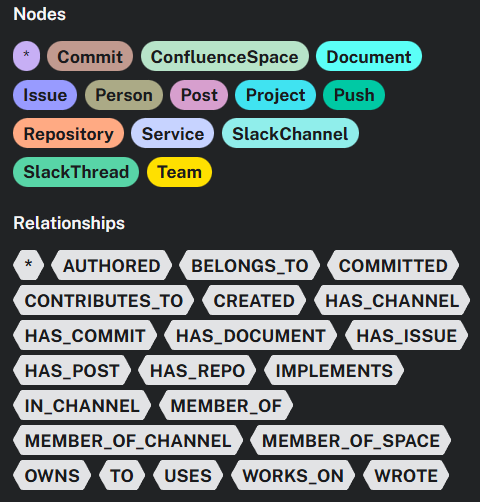
\includegraphics[width=0.8\textwidth]{Figures/nodesANDrelationships.png}
    \caption{Översikt över grafdatabaslösningens entiteter och deras relationer}
    \label{fig:methodology}
\end{figure}

I den fjärde fasen utvecklades systemet enligt den design som skapats i föregående fasen.
Här skrevs koden för MCP servern, integrationen med LLM:en och kommunikationen med databasen och externa systems API:er.
Systemet byggdes iterativt där olika delar utvecklades och testades allt eftersom.

I den femte fasen testades systemen. Här genomfördes olika tester för att besvara de frågor som legat som grund för arbetet.
Här mättes svarstid, antal verktygsanrop, korrekthet och relevans för att komma fram till ett resultat.
 Detta möjliggjorde en analys av skillnaderna mellan de två lösningarna, och därmed besvara forskningsfrågorna och dra en slutsats.

I den sista fasen utvärderades systemet. Här identifierades möjliga ändringar som hade kunnat implementerats i systemen.
Det diskuterades även om framtida forskning och vidare utveckling av systemen. 


\subsection{Utvärderingsmetod}\label{subsec:evalmethod}
Arbetet utvärderas genom att jämföra de två skapade lösningarna för att besvara de forskningsfrågor som identifierats i kapitel \ref{subsec:researchquestion}.
De båda lösningarna kommer att ha tillgång till liknande information, och testas genom att få samma uppsättning frågor som de ska besvara.

För att besvara forskningsfrågorna så kommer det att mätas svarstid, antal verktygsanrop, korrekthet och relevans. 

\subsubsection{Jämförelsens syfte och avgränsningar}

Syftet med studien är inte att genomföra en strikt jämförelse mellan två identiska system, utan att undersöka hur olika sätt att representera organisatorisk information påverkar en LLM:s förmåga att kunna navigera till och hämta rätt information.

Den grafbaserade lösningen utgör studiens huvudsakliga fokus, då den representerar ett alternativt sätt att strukturera och representera information på.

Det är också viktigt att ta hänsyn till att de två lösningarna inte har tillgång till exakt samma information eller informationsrepresentation.
Den grafbaserade lösningen bygger på en strukturerad kunskapsgraf där relationer mellan entiteter är manuellt modellerade för att efterlikna en organisations olika delar.
Den API-baserade lösningen hämtar istället information från specifika och faktiska datakällor.

Eftersom den grafbaserade lösningen är manuellt modellerad betyder det även att all data i den är manuellt skapad och inte verklig, medan den API-baserade lösningen hämtar verklig data från riktiga API:er.

Det betyder att de båda lösningarna skiljer sig från varandra i form av vad data innehåller och hur mycket data som finns i dem. 
Det påverkar tidsmätningen i testerna samt skärmdumparna som finns i \ref{sec:appA}, och detta kommer att diskuteras mer ingående i kapitel \ref{sec:discussion}.


\subsection{Reliabilitet och validitet}\label{subsec:reliabilityvalidity}
\subsubsection{Reliabilitet}
En begränsning i arbetet är att varje testfråga endast besvaras en gång av varje system.
Eftersom LLM:er är icke-deterministiska kan svaret variera mellan körningar \cite{llm_nondeterminism,llm_background_temperature}.
 Detta innebär att resultaten inte nödvändigtvis är fullt reproducerbara.

Svarstiden påverkas dessutom av externa faktorer såsom nätverkshastighet och belastning på LLM:ens API-server,
 vilket gör att tidsmätningarna bör tolkas som indikativa istället för exakta.

\subsubsection{Validitet}
Korrekthetsbedömningen av svaren görs manuellt och innebär därmed ett visst mått av subjektivitet.
För att minska denna subjektiviteten jämförs svaren med information från respektive system för att se till att det är rätt information som hämtats.

Utvärderingen baseras på 15 testfrågor där de två lösningarna har tillgång till olika informationskällor.
Resultaten bör därför ses som något som visar lösningarnas styrkor och svagheter snarare än en definitiv jämförelse av deras prestanda i alla situationer.

